% !TEX TS-program = XeLaTeX
% use the following command:
% all document files must be coded in UTF-8
\documentclass[portuguese]{textolivre}
% build HTML with: make4ht -e build.lua -c textolivre.cfg -x -u article "fn-in,svg,pic-align"

\journalname{Texto Livre}
\thevolume{15}
%\thenumber{1} % old template
\theyear{2022}
\receiveddate{\DTMdisplaydate{2021}{9}{21}{-1}} % YYYY MM DD
\accepteddate{\DTMdisplaydate{2021}{12}{9}{-1}}
\publisheddate{\DTMdisplaydate{2022}{2}{15}{-1}}
\corrauthor{Cláudia Freitas}
\articledoi{10.35699/1983-3652.2022.36213}
%\articleid{NNNN} % if the article ID is not the last 5 numbers of its DOI, provide it using \articleid{} commmand
\runningauthor{Freitas et al.} 
%\editorname{Leonardo Araújo} % old template
\sectioneditorname{Daniervelin Pereira}
\layouteditorname{Leonado Araújo}

\title{Um ‘olhar discursivo’ sobre predicação e gênero: aproximações metodológicas entre \textit{corpus} e discurso}
\othertitle{‘Discourse reading’ predication and gender: putting together  and discourse analysis}
% if there is a third language title, add here:
%\othertitle{Artikelvorlage zur Einreichung beim Texto Livre Journal}

\author[1]{Cláudia Freitas \orcid{0000-0001-6807-8558} \thanks{Email: \url{claudiafreitas@puc-rio.br}}}
\author[1]{Flávia Martins \orcid{0000-0001-6346-2032} \thanks{Email: \url{flaviamrpsilva@gmail.com}}}
\author[1]{Liana Biar \orcid{0000-0002-8673-8668} \thanks{Email: \url{lianabiar@gmail.com}}}
\affil[1]{Pontifícia Universidade Católica do Rio de Janeiro, Departamento de Letras, Rio de Janeiro, RJ, Brasil.}


\addbibresource{article.bib}
% use biber instead of bibtex
% $ biber article

% used to create dummy text for the template file
\definecolor{dark-gray}{gray}{0.35} % color used to display dummy texts
\usepackage{lipsum}
\SetLipsumParListSurrounders{\colorlet{oldcolor}{.}\color{dark-gray}}{\color{oldcolor}}

% used here only to provide the XeLaTeX and BibTeX logos
\usepackage{hologo}

% if you use multirows in a table, include the multirow package
\usepackage{multirow}

% provides sidewaysfigure environment
\usepackage{rotating}

% CUSTOM EPIGRAPH - BEGIN 
%%% https://tex.stackexchange.com/questions/193178/specific-epigraph-style
\usepackage{epigraph}
\renewcommand\textflush{flushright}
\makeatletter
\newlength\epitextskip
\pretocmd{\@epitext}{\em}{}{}
\apptocmd{\@epitext}{\em}{}{}
\patchcmd{\epigraph}{\@epitext{#1}\\}{\@epitext{#1}\\[\epitextskip]}{}{}
\makeatother
\setlength\epigraphrule{0pt}
\setlength\epitextskip{0.5ex}
\setlength\epigraphwidth{.7\textwidth}
% CUSTOM EPIGRAPH - END

% LANGUAGE - BEGIN
% ARABIC
% for languages that use special fonts, you must provide the typeface that will be used
% \setotherlanguage{arabic}
% \newfontfamily\arabicfont[Script=Arabic]{Amiri}
% \newfontfamily\arabicfontsf[Script=Arabic]{Amiri}
% \newfontfamily\arabicfonttt[Script=Arabic]{Amiri}
%
% in the article, to add arabic text use: \textlang{arabic}{ ... }
%
% RUSSIAN
% for russian text we also need to define fonts with support for Cyrillic script
% \usepackage{fontspec}
% \setotherlanguage{russian}
% \newfontfamily\cyrillicfont{Times New Roman}
% \newfontfamily\cyrillicfontsf{Times New Roman}[Script=Cyrillic]
% \newfontfamily\cyrillicfonttt{Times New Roman}[Script=Cyrillic]
%
% in the text use \begin{russian} ... \end{russian}
% LANGUAGE - END

% EMOJIS - BEGIN
% to use emoticons in your manuscript
% https://stackoverflow.com/questions/190145/how-to-insert-emoticons-in-latex/57076064
% using font Symbola, which has full support
% the font may be downloaded at:
% https://dn-works.com/ufas/
% add to preamble:
% \newfontfamily\Symbola{Symbola}
% in the text use:
% {\Symbola }
% EMOJIS - END

% LABEL REFERENCE TO DESCRIPTIVE LIST - BEGIN
% reference itens in a descriptive list using their labels instead of numbers
% insert the code below in the preambule:
%\makeatletter
%\let\orgdescriptionlabel\descriptionlabel
%\renewcommand*{\descriptionlabel}[1]{%
%  \let\orglabel\label
%  \let\label\@gobble
%  \phantomsection
%  \edef\@currentlabel{#1\unskip}%
%  \let\label\orglabel
%  \orgdescriptionlabel{#1}%
%}
%\makeatother
%
% in your document, use as illustraded here:
%\begin{description}
%  \item[first\label{itm1}] this is only an example;
%  % ...  add more items
%\end{description}
% LABEL REFERENCE TO DESCRIPTIVE LIST - END


% add line numbers for submission
%\usepackage{lineno}
%\linenumbers

\begin{document}
\maketitle

\begin{polyabstract}
\begin{abstract}
Este artigo propõe uma sinergia metodológica entre os estudos linguísticos com base em grandes \textit{corpora} e os estudos do discurso, trazendo como contribuição as possibilidades de trabalho com anotação linguística. A análise tem o elemento gênero como operador analítico, selecionando uma de suas dimensões: caracterizações atribuídas a personagens femininas e masculinas. A pesquisa tomou por base um grande acervo composto por mais de 200 obras da literatura brasileira em domínio público (cerca de 5 milhões de palavras). A partir da busca por estruturas linguísticas indicativas de predicação, distinguimos quatro eixos de análise, ampliando um tipo de trabalho que normalmente se restringe aos estudos de caso. Ao longo do artigo, e graças às ferramentas computacionais, alternamos entre lentes que nos afastam e nos aproximam do texto, tentando tirar o melhor proveito de cada uma delas. Por fim, argumentamos que é possível - e desejável - superar as dicotomias quantitativo x qualitativo e conteúdo x discurso.

\keywords{Humanidades digitais \sep Linguística de corpus \sep Mineração de dados textuais \sep Análise de discurso \sep Estudos de gênero}
\end{abstract}

\begin{english}
\begin{abstract}
This paper proposes a methodological synergy between corpus linguistics and discourse studies. We use a literary corpus composed of more than 200 books of Brazilian literature (about 5 million words) and present a quantitative and qualitative analysis that takes the gender element as an analytical operator, selecting one of its dimensions: characterizations attributed to female and male characters. Searching for linguistic structures indicative of predication, we distinguished four axes of analysis (appearance, emotion, character e social role), expanding a type of research that is normally restricted to case studies. Using computational tools, we switch the glasses that bring the text to a close or a distant reading, making the best of each of these perspectives. The results reinforce the idea of female characterization centered on appearance (specifically on beauty), but also signal the importance of taking into account not only the high frequency elements of the corpus.

\keywords{Digital Humanities \sep Corpus linguistics \sep Text mining \sep Discourse analysis \sep Gender studies}
\end{abstract}
\end{english}
% if there is another abstract, insert it here using the same scheme
\end{polyabstract}

\section{Introdução}\label{sec-intro}
Desde meados dos anos 2000 que os estudos linguísticos vêm se beneficiando de métodos e ferramentas desenvolvidos no contexto de uma linguística empírica que toma por base grandes corpora linguísticos \cite{sampson2002, santos2008, mcenery2011, finatto2018}. No entanto, boa parte dos trabalhos realizados está voltada para a dimensão léxico-gramatical da língua, seja no contexto da lexicografia (monolíngue ou bilíngue), da caracterização de gêneros textuais ou do ensino de uma língua estrangeira. Por outro lado, \textcite{baker2008} propõem uma “sinergia metodológica” entre o uso de \textit{corpus} e análise crítica do discurso, analisando o discurso sobre refugiados e imigrantes na mídia impressa do Reino Unido a partir de um \textit{corpus} de 140 milhões de palavras.  

O que propomos neste artigo, na esteira do que fazem \textcite{baker2008} no contexto europeu, é que o mesmo tipo de sinergia metodológica possa não apenas ser concebido, mas também aprofundado, no âmbito da análise discursiva brasileira\footnote{Entre a submissão e o aceite do presente artigo, tivemos notícia de uma empreitada semelhante à nossa. \textcite{ramalho2021} tecem considerações metodológicas sobre uso de software em pesquisa discursiva. As autoras descrevem especificamente o uso do programa NVivo, capaz de organizar, codificar em categorias e cruzar dados textuais de diferentes fontes a escolha das pesquisadoras.}. Dados os mais de 10 anos que nos separam, é razoável poder contar não apenas com a indicação de frequência e de coocorrência entre termos, como fazem \textcite{baker2008, baker2013}; \textcite{strom2017} e \textcite{friginal2020}, dentre outros, mas, principalmente, com as possibilidades que resultam da adição de anotação linguística nos corpora, permitindo mais profundidade na análise dos dados. Escolhemos para as explorações e análises um tema caro à análise discursiva, os estudos de gênero, selecionando uma de suas dimensões: caracterizações atribuídas a mulheres e homens, utilizando um grande acervo de obras da literatura brasileira.

\textcite{smith2014}, em uma pesquisa sobre representatividade de gênero na indústria cinematográfica, trazem os seguintes dados após a análise de personagens femininas em filmes \textit{blockbuster} produzidos em 11 países: apenas 31\% dos papéis com alguma fala são interpretados por personagens femininas; somente 23\% dos protagonistas são mulheres; independente do país, personagens femininas destacam-se pela aparência (mulheres têm 5 vezes mais chances do que os homens de receberem comentários baseados na aparência). No que se refere à dimensão profissional, o estudo também mostra a desigualdade quanto à carreira das personagens: para cada profissional mulher, há 7 homens com profissões. Quando reconhecemos a importância da representatividade e a influência da mídia na criação e na manutenção de viés, a relevância não apenas dos resultados, mas também do tipo de pesquisa realizada, é evidente.

Ao escolher como fonte obras literárias e ao utilizar ferramentas de anotação produzidas pela Linguística Computacional, também nos aproximamos das Humanidades Digitais, uma abordagem para as Humanidades baseada em princípios de abertura de dados, compartilhamento e interdisciplinaridade. Se, hoje, as Humanidades Digitais vão além do trabalho com acervos textuais, historicamente a área surge vinculada a estudos literários (veja-se \textcite{santos2019} para uma panorâmica da relação entre \textit{corpus} e humanidades digitais, com foco na língua portuguesa). Nesse contexto, uma abordagem que vem se popularizando é a \textit{leitura distante (distant reading)}. O termo foi cunhado por Moretti “um pouco por brincadeira e um pouco não” \cite[p. 8]{moretti2005} para fazer referência uma tomada de distância providencial, que faz da distância não um obstáculo, mas uma forma específica de conhecimento. “A distância faz com que se vejam menos detalhes, mas faz com que se observem melhor as relações, os padrões, as formas” \cite[p. 8]{moretti2005}. Temos, portanto, na leitura distante, uma estratégia que claramente privilegia uma abordagem macroscópica e quantitativa (veja-se \textcite{moretti2019} para uma visão panorâmica e crítica mais recente).

No presente trabalho, articulamos o que poderia ser chamado de uma leitura distante com uma leitura aproximada dos dados. Tomamos distância para ver o todo (e o todo é definido segundo a perspectiva de quem vê, ressaltamos) e, em seguida, aproximamo-nos, para ver com detalhes o que, de longe, pareceu-nos relevante.

Assumindo, de maneira bastante simplificada, uma distinção entre teoria e método, de um ponto de vista metodológico nos alinhamos com estratégias que utilizam grandes dados para análise, explorando potencialidades deste outro ponto de vista, disponível quando podemos “ler” grandes volumes de texto de uma maneira não-linear \cite{freitas2017, paixao2013}. De um ponto de vista teórico, o que sugerimos, aqui, a despeito do desenvolvimento de um campo de estudo que se fundou em posições excludentes como “quantidades” versus “qualidades” e “conteúdo” versus “discurso”, é que qualquer abordagem que esteja dentro do guarda-chuva heterogêneo que se convencionou chamar de “análise de discurso” poderia se beneficiar deste tipo de abordagem.

Desenvolveremos o argumento deste artigo em três etapas: em primeiro lugar, nos debruçaremos brevemente sobre as dicotomias quantitativo x qualitativo; conteúdo x discurso, apontando para os modos como elas podem ser relativizadas em benefício da articulação aqui proposta. Em segundo lugar, exemplificaremos as possibilidades de trabalho tomando como objeto de exploração obras da literatura brasileira em domínio público (majoritariamente a literatura do século XIX e início do século XX), em um \textit{corpus} com cerca de 5 milhões de palavras, o \textit{corpus} OBras \cite{santos2018}. Esse \textit{corpus} foi anotado morfossintaticamente por um analisador automático, o que permite pesquisas mais complexas do que padrões de coocorrência. Especificamente, nos dedicamos a explorar padrões léxico-sintáticos indicativos de predicação, a fim de obter caracterizações de personagens em nosso acervo. Por fim, a partir do nosso exemplo de análise, procuraremos demonstrar como essa exploração pode embasar um ponto de vista fértil, que chamaremos de “um olhar discursivo” sobre os dados.

Nosso objetivo é duplo: por um lado pretendemos apresentar uma proposta de agenda analítica que constrói suas reflexões a partir de um exemplo “piloto” de análise, por outro, trazemos para a discussão os resultados preliminares de uma análise da caracterização de personagens em obras literárias brasileiras tomando a categoria gênero como eixo de análise.

\section{Algumas notas sobre abordagens quantitativas e qualitativas, conteúdo e discurso}\label{sec-2}
Ainda que a pesquisa com grandes corpora seja associada a análises quantitativas, em boa parte das Humanidades a dimensão quantitativa é o polo a ser evitado na dicotomia quantitativo \textit{versus} qualitativo. Discordamos integralmente desse posicionamento, não por defender a superioridade do método quantitativo – pelo contrário, nossa aposta está na dissolução da dicotomia. A esse respeito, gostaríamos de apresentar aqui dois argumentos relacionados.

Lembramos, com \textcite{santos2014}, que, para contar/quantificar, é preciso, em primeiro lugar, qualificar (o objeto da contagem precisou ser reconhecido enquanto tal, precisou ser qualificado), o que reforça nosso ponto de que a polarização pressuposta é apenas mais uma dentre tantas outras a serem evitadas quando não aderimos a posições logocêntricas. Concordamos, também, com \textcite{leite2015} quando lembram que assim como desenvolvimentos tecnológicos permitiram disponibilizar “um quantitativo informacional inédito na história da humanidade, também possibilitaram a criação de ferramentas que viabilizam abordagens inovadoras” e que “a irrepetibilidade do acontecimento social contingente (...) pode se beneficiar da perspectiva quantitativa que salienta os casos singulares” \cite[p.~141]{leite2015}.

Assim como números não são neutros, não o são nem os dados, nem as tecnologias. No caso específico da pesquisa com grandes corpora, não nos alinhamos com um posicionamento segundo o qual os dados emergem do \textit{corpus}, fruto de tecnologias assépticas, prontos para serem analisados por uma pesquisadora–observadora neutra ou bem treinada: são, antes, objetos construídos segundo a perspectiva de quem pesquisa. Esse é o nosso segundo argumento. Quando nos referimos a tradições qualitativas e quantitativas, estamos tratando de \textit{escolhas metodológicas}. A tradição nas ciências humanas tende a associar opções quantitativas a paradigmas epistemológicos objetivistas, preocupados em desvelar e medir relações entre variáveis e, inversamente, os métodos qualitativos a práticas interpretativas situadas que localizam quem pesquisa (sua história, posições, lugares de fala) como parte constitutiva da produção do conhecimento \cite{denzin2006}. Essa é uma associação arbitrária. Naturalmente, métodos de análise sempre responderão a filiações de ordem onto-epistemológica, em que o que está em jogo é o que se pensa sobre a natureza do “real” e sobre os modos e as possibilidades de se construir conhecimento sobre ele nas atividades de pesquisa. Nesse sentido, é perfeitamente possível \textit{contar} sem ilusão de objetividade, desde que de dentro da “cosmovisão” filosófica relativista. Da mesma maneira, nem toda índole qualitativo-interpretativa prescinde do primado da neutralidade e está livre de pretensões \textit{reveladoras} de verdades científicas.

No terreno dos trabalhos com corpora, a anotação linguística exemplifica tanto o caráter interessado das tecnologias como a facilidade com que este interesse se disfarça de naturalidade ou objetividade.  Ainda que frequentemente realizada de maneira automática, a anotação é uma atividade interpretativa, que envolve a adição de informação linguística a porções de texto, levando em conta o contexto e segundo certos pressupostos de análise (explicitados nas diretivas de anotação). Mesmo que a anotação associada à dimensão morfossintática da língua seja bastante frequente – e a longa tradição da metalinguagem gramatical contribui para a estabilidade de certas análises, que passam a ser vistas como objetivas – anotações de natureza pragmática e discursiva, dentre outras, têm comparecido em trabalhos de interesses diversos \cite{ide2017}.

A anotação é uma atividade de classificação ou categorização. Por meio dela, organizamos os dados (palavras ou segmentos maiores de texto) em classes (etiquetas de anotação ou \textit{tagset}), conforme certos interesses (os interesses que motivam a própria anotação). Quando inserimos a nossa interpretação nos dados por meio da anotação, o que temos, em grande escala, é essa mesma interpretação. Trata-se, assim, de uma maneira de concatenar a dimensão qualitativa à quantitativa. Afinal, o que contamos são análises (qualitativas) baseadas nos mesmos critérios de interpretação (explicitados nas diretivas de anotação e verificados por meio da concordância interanotadores).

No terreno dos estudos discursivos, tanto os de origem francesa \cite[por exemplo]{maingueneau2015} quanto os de origem anglo-saxã \cite[por exemplo]{fairclough1992}, é bastante conhecida a distinção entre o que chamamos aqui genericamente de "análise de discurso" e "análise de conteúdo" \cite{bardln1977}. De acordo com Bardin, a análise de conteúdo é uma técnica para se obter, por meio de procedimentos sistemáticos, objetivos e descritivos, indicadores para inferências em relação ao contexto de produção e recepção de textos. Esses procedimentos incluem codificação, classificação e análise de frequência de certos itens e o objetivo é encontrar ordem na desordem aparente de um conjunto de dados textuais, segundo certos critérios. Disputando espaço com essa técnica de leitura de textos, as análises de discurso, seja qual for a vertente\footnote{Embora sejam muitas as vertentes abrigadas sob o rótulo guarda-chuva de “estudos do discurso”, e as diferenças entre elas sejam importantes, neste artigo optamos por não nos filiar a uma corrente específica, mas sublinhar o que necessariamente compõe uma perspectiva discursiva em termos gerais, ou seja, apresentar um núcleo comum às várias vertentes. A seguir, faremos referência a conceitos, autores e autoras oriundos de tradições diversas, e fazemos isso sem ignorar suas distintas origens teóricas. Nosso objetivo é mostrar que a sinergia discurso-\textit{corpus} aqui proposta pode beneficiar igualmente diferentes tradições. Uma exposição sobre os afastamentos e as aproximações possíveis entre as diferentes correntes de análise de discurso extrapolaria o escopo do presente artigo, mas pode ser preliminarmente consultada em \textcite{oliveira2013}.}, preocupam-se em se distinguir de sua oponente em termos de concepção de ciência e de linguagem \cite{rocha2005}. Ainda segundo os autores, enquanto analistas de conteúdo apostam em desenvolvimentos de técnicas para extração de conteúdo, confiando em certa transparência da linguagem, os analistas de discurso, por sua vez, desprezam a parafernália tecnicista usada a pretexto de garantir validação e cientificidade e desafiam uma concepção ingênua de autoria individual cega para as complexidades e efeitos da comunicação humana e da construção de sentido, especialmente no que diz respeito às condições de produção e circulação dos discursos. De modo geral, analisar discurso significa produzir interpretações sobre o uso da linguagem que o relacione com seu contexto socialmente situado, com sua emergência sócio-histórico-cultural e com outros discursos que o precedem e sucedem. Sobretudo, uma perspectiva discursiva aposta em uma dimensão performativa da linguagem, isto é, na sua possibilidade de moldar a realidade social no lugar de simplesmente representá-la.

Apesar de o tipo de trabalho que desenvolvemos nos aproximar aparentemente da análise de conteúdo (compartilhamos da adoção de procedimentos sistemáticos e o uso intenso de computadores, por exemplo), tal convergência é apenas superficial. Bebemos da mesma fonte que as análises discursivas no que toca às suas referências não-logocêntricas, o que se manifesta, por exemplo, na descrença quanto à suposta neutralidade das tecnologias. Nessa visada, a dispersão bruta dos dados não é pensada como algo que deve ser arrumado em benefício da norma, mas merece por si uma perspectiva que a privilegie. A própria ideia de arrumação, aliás, é sem sentido: não buscamos “a ordem na desordem aparente” porque esta ordem não existe, mas buscamos, sim, a construção de alguma ordem (isto é, de alguma estrutura), contingente, parcial, afetada pelas lentes socioculturais de quem pesquisa, mas capaz de engendrar as análises para as questões que nos parecem pertinentes.

Enquanto método, é difícil afirmar que a maneira pela qual manipulamos grandes corpora tem diferenças significativas com modelo de análise de conteúdo de \textcite{bardln1977}. Pelo contrário, se desconsideramos as tecnologias e recursos de que dispomos hoje, as aproximações são evidentes. Justamente porque as aproximações são incontestáveis, demoraremos um pouco aqui, a fim de deixar clara nossa proposta e evitar futuros mal-entendidos. Concordamos, por exemplo, quanto à utilização de procedimentos sistemáticos, mas divergimos não apenas quanto à sua suposta objetividade, mas também na maneira de operar com tais procedimentos. A categorização, por exemplo, é um procedimento central na análise de conteúdo de \textcite{bardln1977} e na nossa. Mas a maneira de encará-la reflete diferenças profundas.

Em contraponto à afirmação de que "convém classificar as unidades de significação criando categorias, introduzindo uma ordem suplementar reveladora de uma estrutura interna” \cite[p. 55]{bardln1977}, preferimos dizer que introduzimos uma ordem, que não é nem suplementar ou reveladora, mas que permite criar narrativas capazes de jogar luz sobre nossas práticas.  Para nós, a categorização – bem como a anotação de \textit{corpus} – não revela, mas constrói. Essa crença na possibilidade de uma categorização motivada por critérios extra-humanos, posto que o bom analista de conteúdo seria aquele treinado para evitar a subjetividade, subjaz às características positivas das categorias, e que para nós são, por outro lado, alvo de críticas: a \textit{exclusão mútua}, a \textit{homogeneidade} e a \textit{fidelidade}.

Nesse ponto, nossas divergências têm consequências práticas para a maneira como estruturamos a análise: a \textit{exclusão mútua} dá lugar à \textit{classificação múltipla}; a \textit{homogeneidade} (supostamente natural) dá lugar ao reconhecimento de se tratar de uma \textit{homogeneidade construída}; e a \textit{objetividade} dá lugar ao \textit{consenso}, à convergência de análises. A \textit{fidelidade}, outra qualidade tida como positiva, é necessária à análise de conteúdo a fim de evitar “distorções devidas à subjetividade dos codificadores e à variação dos juízos” \cite[p. 120]{bardln1977}. Novamente, nossa posição é diametralmente oposta. A distorção é inerente ao processo de categorização, não há como evitá-la. Igualar o diferente, por meio da categorização, é uma distorção; categorizar é distorcer.

\section{Metodologia}\label{sec-3}
Todo o trabalho de exploração foi feito sobre o OBras (acrônimo de Obras Brasileiras), um \textit{corpus} criado e mantido pela Linguateca\footnote{A Linguateca é um centro que se dedica, desde 1998, a criação, desenvolvimento e disponibilização de infra-estrutura para o tratamento computacional da língua portuguesa. Veja-se \url{http://www.linguateca.pt} e \textcite{santos2019}.}, que contém obras da literatura brasileira que já estão em domínio público. O OBras é um \textit{corpus} dinâmico e continha, na versão 5.3 (versão sobre a qual trabalhamos), 223 obras publicadas entre 1807 e 1977, de 25 autores. Aqui já se vislumbra uma vantagem da sinergia proposta, que é a de lidar com toda essa quantidade de texto de modo relativamente rápido.

Cada obra contém, além de um identificador único, metadados relativos ao gênero literário (conto, romance, crônica etc.) e, no caso dos romances, informações relacionadas à escola literária (Realismo, Romantismo, Naturalismo etc.)\footnote{Veja-se a página do OBras para mais informações: \url{https://www.linguateca.pt/OBRAS/OBRAS.html}}. Todo o material foi anotado morfossintaticamente pelo analisador PALAVRAS \cite{bick2000}, semanticamente pela equipe da Linguateca e está público e disponível para uso, tanto para download como para pesquisa linguística, por meio da interface de acesso AC/DC\footnote{O AC/DC é um serviço criado e mantido pela Linguateca, que permite acessar, em uma única interface \textit{on-line} e sem necessidade de cadastro ou registro, uma coleção de corpora de língua portuguesa, nas variantes do Brasil, Portugal (majoritariamente), Angola e Moçambique, de gêneros diversos e períodos diversos. Todo o material é público e contém anotação morfossintática e semântica. O material disponível pelo AC/DC é dinâmico e contém atualmente mais de 1 bilhão de palavras. Mais informações na página do projeto: \url{https://www.linguateca.pt/ACDC/}}. Utilizamos todas as 223 obras da versão 5.3, das quais apenas três foram escritas por mulheres – \textit{Úrsula} (1859), romance de Maria Firmina dos Reis, considerado o primeiro romance escrito por uma mulher negra no Brasil, e \textit{A falência} (1901) e \textit{A viúva Simões} (1895), ambos de Júlia Lopes de Almeida. Temos, então, em nossas mãos, o que pode ser considerado o cânone literário brasileiro de um período de 170 anos, que permite explorar o olhar da elite brasileira dos séculos XIX e XX, composta essencialmente por homens brancos – exceto por Lima Barreto e Machado de Assis. A presença de apenas duas mulheres na lista de autores é, como se já poderia esperar, um dado sobre o lugar da mulher na sociedade no período selecionado\footnote{Tal (des)proporção entre escritores e escritoras, como se pode imaginar, não é específico do OBras. De acordo com \textcite{santos2014}, a Biblioteca Nacional tem catalogadas trinta e cinco mulheres que desenvolveram publicações no século XIX e início do século XX, o que corresponde a 2.59\% dos escritores do período.}, ponto este que retomaremos na seção 5.

Boa parte do trabalho inicial com grandes corpora pode consistir em uma exploração livre de possibilidades (um estudo exploratório). De início não se sabe bem o que se está procurando – ou, não há, ainda, uma pergunta bem definida. Trata-se de um estudo que “procura correlações, experimenta classificações, identifica conjuntos [...] abre sendas, identifica lugares de interesse (para lá voltar ou para outros lá irem)” \cite[p. 49]{santos2008}.

Começamos por explorar questões de gênero, que nos pareceu um analisador produtivo para se falar das relações entre sociedade (ou gênero) e discurso. Reconhecemos, no entanto, que quando o objeto de estudo é uma construção teórica como \textit{sociedade}, um \textit{corpus}, ainda que contenha enunciados integrais no âmbito do texto, é apenas uma amostra\footnote{Em oposição, por exemplo, à ideia de \textit{corpus} como um acervo, comum nas Humanidades Digitais, quando o \textit{corpus} deixa de ser amostra para ser o objeto: todas as obras de um determinado autor, por exemplo.}. Em seguida, ajustamos o foco analítico para encontrar caracterizações de personagens masculinas e femininas. Buscamos por padrões léxico-sintáticos que indicassem a presença do que chamaremos aqui, em termos amplos, de predicação, em nosso caso, predicação humana\footnote{A predicação é uma relação: se há alguém sendo predicado/qualificado, há alguém responsável pela predicação. Na literatura, quem predica não é o autor – predicações são feitas pelo narrador ou pelas próprias personagens.}. Especificamente, buscamos pelas seguintes estruturas sintáticas: predicativo do sujeito, aposto e adjuntos adnominais\footnote{Utilizamos uma metalinguagem tradicional e no apêndice indicamos como cada estrutura pode ser buscada na interface do AC/DC, para que a comunidade interessada possa não apenas reproduzir os resultados, se assim o desejar, mas também avançar com suas próprias pesquisas.} de substantivos, comuns ou próprios, que representem mulheres e homens (moço/moça, menino/menina, homem/mulher, ele/ela...). O que buscamos, portanto, são manifestações gramaticais da ideia mais geral de predicação e de qualificação, quando aplicadas a pessoas. A \Cref{tbl01} traz exemplos de cada uma das estruturas de interesse.


\begin{table}[htpb]
\caption{Estruturas sintáticas usadas para buscar predicação humana no \textit{corpus}.}
\label{tbl01}
\begin{tabular} {p{4cm} p{9cm}}
\toprule 
Estrutura & Exemplo \\
\midrule
Predicativo do sujeito & id="Histórias\_sem\_Data prosa:conto MdA 1884": Já disse que \textbf{Eulália} era ainda \textbf{bonita}. \\
\midrule
Aposto & d="Quincas\_Borba Prosa:romance MdA 1886 realismo masc ": Maria Benedita era o nome da avó dela, afilhada de \textbf{Luís de Vasconcelos}, o \textbf{vice-rei}. \\
\midrule
Modificadores (adjuntos adnominais) de mulheres e homens & id="A\_serpente\_de\_bronze prosa:conto HC 1921": Criemos as meninas com decoro, vestindo-as com discrição, e teremos \textbf{moças discretas}, \textbf{pudicas}, \textbf{decorosas}, \textbf{ciosas} do seu corpo e dos seus encantos. \\
\bottomrule
\end{tabular}
\source{Elaboração própria.}
\end{table}

Este procedimento garante que as palavras encontradas estão sendo usadas em um contexto de predicação humana – e isto é diferente, por exemplo, de um trabalho com base em um léxico, ainda que o léxico contivesse exatamente as mesmas palavras, pois nem toda ocorrência de \textit{bonita}, \textit{nova} ou \textit{pura} qualifica pessoas. Assim, o conteúdo das listas que apresentaremos a seguir, embora traga apenas palavras isoladamente, está contextualizado, graças à anotação sintática. Uma outra vantagem de lidar com os padrões está, portanto, na própria estabilização de sentidos que operam. Temos acesso ao contexto, apenas o escondemos – mas podemos torná-lo visível a qualquer momento, voltando às linhas de concordância: aproximação e distanciamento. No entanto, reconhecemos que nem todas as predicações humanas se manifestam nos padrões que exploramos, e a relativa baixa abrangência – em oposição à alta precisão – é uma limitação deste tipo de abordagem \cite{hearst1992}, até hoje utilizada na extração automática de informação em textos\footnote{As métricas de precisão e abrangência são comuns na recuperação de informação e na linguística computacional. Uma alta precisão indica que, dos elementos identificados automaticamente, a maior parte foi corretamente identificada; uma alta abrangência indica que, de todos os elementos (corretos) que se poderia identificar automaticamente, a maior parte foi identificada. Deste modo, uma alta precisão e baixa abrangência indicam que aquilo que é identificado pelo padrão está correto na maioria das vezes, mas há outros casos de predicação humana que não são detectados pelo padrão.}. Ainda assim, a estratégia é produtiva e seguimos com ela.   

Outra aparente limitação da abordagem está na dificuldade de perceber certos detalhes que nem sempre estão desprovidos de importância, como o caso das negações. Ou seja, olhando apenas para as listas, é difícil garantir que aquele elemento predicador de fato estava ali para caracterizar uma personagem e não para, por exemplo, negar essa caracterização. Aqui, respondemos de duas maneiras: por um lado, esta “perda” faz parte do jogo das grandes quantidades, e a ideia não é negar que casos assim possam aparecer, mas, sendo pouco frequentes (no padrão utilizado), irão se diluir. Temos sempre, nesse tipo de trabalho, \textit{tendências}. E as linhas de concordância permanecem disponíveis para analisar cada instância e cada situação. Por outro lado, a própria expressão de busca que utilizamos minimiza, especificamente, a ocorrência de negações.        

\section{Resultados iniciais}\label{sec-normas}
As expressões utilizadas encontram um total de 3.862 predicações, 60\% delas atribuídas a personagens masculinas, e 40\%, a personagens femininas. A primeira constatação a partir desses números é que se descrevem mais personagens masculinas do que femininas – uma consequência de haver mais personagens masculinas do que femininas nas obras que compõem o \textit{corpus}. De fato, quando consideramos a distribuição dos personagens por gênero, a proporção é praticamente a mesma: 60\% dos nomes próprios que se referem a pessoas são masculinos.

Em seguida, adotamos uma perspectiva qualitativa e quantitativa, simultaneamente, a fim de detalhar quais são os predicadores mais comuns por gênero. A \Cref{tbl2} lista os 10 predicadores (lemas\footnote{O lema corresponde à forma de citação – infinitivo para os verbos, masculino e singular para adjetivos, singular para substantivos.}) mais frequentes por gênero, indicando a frequência com que ocorrem\footnote{Por meio da interface AC/DC, temos acesso não apenas às linhas de concordância, mas também à informação de distribuição, de grande relevância quando estamos diante de um material vasto.}.

\begin{table}[htbp]
\caption{Distribuição dos lemas das 10 predicações mais frequentes, por gênero.}
\label{tbl2}
\centering
\begin{tabular}{llll}
\toprule
\multicolumn{2}{l}{Pred. masculinas} & \multicolumn{2}{l}{Pred. femininas} \\ \midrule
sério     & 43 & bonito   & 113  \\ 
bom       & 41 & belo     & 38   \\ 
alto      & 33 & amado    & 36   \\
rico      & 28 & pálido   & 28   \\ 
honesto   & 22 & formoso  & 24   \\ 
digno     & 21 & feliz    & 19   \\ 
magro     & 21 & rico     & 18   \\ 
pobre     & 21 & honesto  & 17   \\ 
solteiro  & 20 & casado   & 17   \\ 
inteligente & 19 & bom    & 16   \\ 
\bottomrule
\end{tabular}
\source{Elaboração própria.}
\end{table}

Nas predicações masculinas, não há nenhum grande destaque, e vemos uma distribuição relativamente equilibrada das predicações. Nas predicações femininas, \textit{bonita} é o grande destaque (porque é muito mais frequente que as demais predicações) e se repete muito mais que a predicação masculina mais comum: temos 113 ocorrências de \textit{bonita}, e 43 ocorrências de \textit{sério}. Os números – mais especificamente, a repetição - indicam a previsibilidade em uma representação do corpo feminino valorizado (o corpo feminino “bonito”), o que é reforçado pela segunda predicação feminina mais frequente (\textit{bela}), também referente à aparência. Somando-se \textit{bonita}, \textit{bela} e \textit{formosa} (posição 5), temos que a beleza feminina responde por 53\% das caracterizações femininas da \Cref{tbl2}, em uma situação muito diferente da caracterização masculina, na qual a aparência aparece na 3ª e 7ª posição (\textit{alto} e \textit{magro}, respectivamente), e responde por apenas 20\% das caracterizações masculinas.  De fato, levando em conta apenas as palavras da \Cref{tbl2}, a caracterização da aparência feminina aparece 4 vezes em 10 (\textit{bonita}, \textit{bela}, \textit{pálida}, \textit{formosa}), e a da aparência masculina, apenas duas vezes (\textit{alto} e \textit{magro}). Além disso, 3 das 4 caracterizações femininas dizem respeito à beleza, atributo feminino socialmente valorizado, e o que não aparece nas caracterizações masculinas.

Já a predicação masculina incide sobretudo no caráter (\textit{sério}, \textit{bom}, \textit{honesto}, \textit{digno} e \textit{inteligente}) e no enquadramento social (\textit{rico}, \textit{pobre}, \textit{solteiro}).  Quanto ao caráter, mulheres também são \textit{honestas} e \textit{boas}; quanto ao enquadramento social, mulheres são \textit{casadas} e \textit{ricas} e só. \textit{Feliz} e \textit{amada}, que predicam estados emocionais/afetivos, são caracterizações femininas; por outro lado, não há predicações dessa natureza associadas às personagens masculinas, ao menos entre as 10 caracterizações mais frequentes. Em resumo, considerando apenas as 10 predicações mais frequentes por gênero, vemos que a caracterização feminina está direcionada sobretudo à aparência (especificamente à beleza do corpo), ao passo que a caracterização masculina enfatiza principalmente traços de caráter e personalidade. A dimensão afetiva, nessa pequena amostra, não comparece nas caracterizações masculinas.

No entanto, a análise se baseou apenas nas 10 predicações mais frequentes por gênero, o que é muito pouco quando dispomos de quase 800 predicações masculinas diferentes e pouco mais de 500 predicações femininas diferentes. Quando voltamos aos dados e acessamos a lista completa de predicações masculinas e femininas, salta aos olhos a variedade lexical: considerando apenas as predicações femininas, enquanto a palavra mais frequente (posição 1) possui 113 ocorrências (\textit{bonita}); a palavra na posição 10 possui apenas 16 ocorrências. Seguindo com a lista, temos 51 palavras com 3 ocorrências; 92 palavras com apenas duas ocorrências e, para finalizar, temos 433 palavras com apenas uma única ocorrência em todo \textit{corpus}. Em outras palavras, no que se refere às predicações femininas, 64\% delas aparece uma única vez. A situação é a mesma na predicação masculina, em que 674 (69\%) das predicações são ocorrências únicas. Esta distribuição, com uma grande parcela de casos raros e que evidencia o excepcional e o singular como maioria, é esperada quando observamos a língua de um ponto de vista quantitativo. Especificamente, a distribuição remete à chamada lei de Zipf e ao fenômeno da cauda longa, assim nomeado devido ao formato do gráfico produzido (para explorações linguísticas da lei de Zipf, veja-se, por exemplo, \textcite{manning1999}, \textcite{santos2008}, \textcite{santos2014}, \textcite{freitas2017}\footnote{Segundo a lei de Zipf, a frequência de um elemento é inversamente proporcional a sua classificação: um elemento na posição 2 terá metade da frequência do elemento na posição 1; o elemento na posição 3 terá um terço da frequência do elemento na posição 1, e assim por diante.}.  

\begin{figure}[htbp]
 \centering
 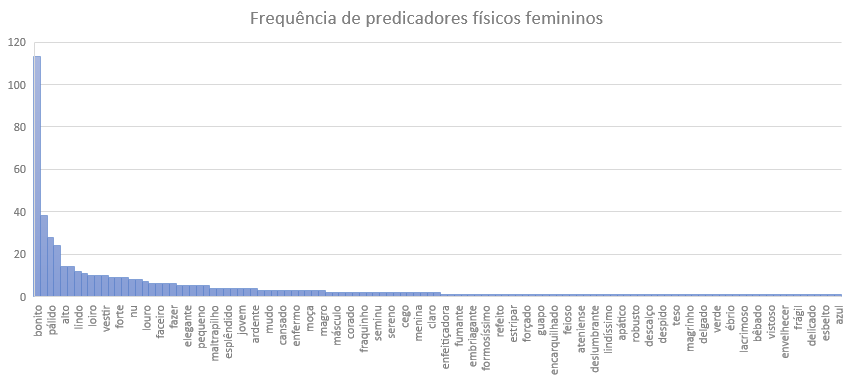
\includegraphics[width=\textwidth]{Fig1.png}
 \caption{Distribuição das predicações femininas, exemplificando a cauda longa.}
 \label{fig1}
 \source{Elaboração própria.}
\end{figure}

Para os objetivos deste trabalho, a cauda longa evidencia a impossibilidade de generalização – e, consequentemente, de atribuição de sentido – a partir de uma lista na qual mais da metade das palavras aparece apenas uma vez. Ou seja, se desejamos observar padrões, a cauda longa é um obstáculo. Por outro lado, ignorar as ocorrências singulares e lidar apenas com as formas mais frequentes tem como consequência dispensar mais de metade dos dados. A \Cref{fig1} ilustra o fenômeno usando os resultados da predicação feminina. Como vemos, temos algumas poucas palavras de frequência alta, algumas de frequência média e uma imensa parcela com uma frequência muito baixa, formando uma “cauda longa” no gráfico.

\subsection{Ajuste no foco: igualar o diferente para atribuir sentido}\label{sec-conduta}
De modo a sair deste impasse e atribuir sentido ao conjunto de dados, distribuímos as predicações nos quatro eixos utilizados na análise preliminar: \textit{aparência}, \textit{emoção}, \textit{papel social} e \textit{caráter}. São eixos/categorias criadas analiticamente a partir dos dados e motivadas por nossos interesses de pesquisa – a caracterização humana.

A distribuição por eixos – ou classes de análise – é \textit{uma} maneira de estruturar e atribuir sentido às ocorrências únicas. Retomando a proposta da análise de conteúdo (AC), trata-se certamente de uma maneira de organizar os dados, mas diferentemente do que prevê a AC, de organizá-los conforme os nossos interesses, em oposição a uma organização correta ou natural.

Da perspectiva da leitura distante, o que vemos sem a distribuição por eixos é bastante limitado. Ao trabalhar com padrões manifestos exclusivamente a partir das quantidades, acabamos prestando atenção naquilo que está mais diretamente observável. Como vimos com a cauda longa, porém, uma boa parte dos fenômenos da língua não se repete e uma vez que aquilo que não se repete não forma padrões, não podem ser \textit{lidos} de longe. O que fazemos aqui, por meio da classificação, é distribuir as palavras em classes pré-estabelecidas (os quatro eixos de análise), criando similaridades que, então, associadas à frequência, criarão padrões. A classificação/anotação, assim, atribui sentidos mais gerais às ocorrências únicas, igualando-as a partir do momento em que passam a pertencer a uma mesma categoria, ou seja, \textit{bonito} e \textit{feio} são tornados iguais porque ambos são elementos da classe \textit{aparência}.

Com isso, a anotação insere camadas na leitura distante, permitindo não apenas ter a distância como aliada, mas também articular leitura distante e aproximada, uma vez que passamos a ver padrões relativos à interpretação.  

A distribuição de todas as palavras das listas em algum dos quatro eixos foi feita, manualmente, por duas autoras deste artigo e serviu ainda como um exercício piloto para a anotação semântica de todo o acervo literário disponível na Linguateca\footnote{O material está público e pode ser consultado em \url{http://www.linguateca.pt/Gramateca/PredicacaoHumana.html}}. Ao longo do processo, foram raros os casos que não se enquadraram em nenhum dos eixos, seja porque se tratava de algum outro tipo de predicação, ou porque a anotação automática estava errada\footnote{Ao final do processo, foram descartadas cerca de 10\% de predicações fruto de erro na análise automática. O processo de análise e classificação está detalhadamente descrito em \textcite{silva2021}.}

Nem sempre uma palavra se encaixa perfeitamente em um eixo/categoria, mas se de alguma maneira a classificação for aceitável, ela será feita. Estamos cientes de que a atividade de categorização é decorrente de um processo de abstração, que envolve a simplificação e a eliminação das diferenças em nome de uma homogeneização \textit{construída} (todas as palavras se “igualam” quando passam a pertencer a uma mesma categoria/eixo).

Outra característica do nosso processo de classificação é a não exclusividade, isto é, um mesmo predicador pode participar de dois ou mais eixos, simultaneamente, e isso não é um problema. Pelo contrário, tomamos a vagueza como propriedade das línguas e do sentido e mesmo em contextos específicos os significados podem ser múltiplos. Nas frases a seguir, indicamos as classes atribuídas a cada uma das palavras em negrito, e a classificação múltipla não indica que os sentidos das duas (ou mais) classes referidas estão igualmente presentes em todas as ocorrências:

\begin{itemize}
    \item “Nem os moços \textbf{valentes}\textsubscript{[emo \& caráter]}, nem os senhores respeitáveis, nem os jornalistas vão sequer à delegacia.” (A Alma Encantadora das Ruas)
    \item “Eugênio, \textbf{trêmulo}\textsubscript{[aparência \& emo]}, confuso e de olhos no chão deixou cair sobre sua cabeça toda esta tremenda trovoada.” (O Seminarista)
\end{itemize}

A etapa de classificação das palavras é, assim, central para as análises subsequentes derivadas do \textit{corpus}. Nos trabalhos de anotação de corpora, a qualidade e consistência das análises, isto é, da anotação, é avaliada por meio da concordância interanotadores \cite{artstein2017}. A concordância é uma maneira de avaliar o grau de convergência das interpretações humanas na anotação de um \textit{corpus} e, por isso, um alto índice de concordância é indicativo da qualidade da anotação de um \textit{corpus}. A hipótese subjacente é que se diferentes pessoas, seguindo as mesmas instruções (em nosso caso, uma breve apresentação das classes \textit{aparência}, \textit{afeto}, \textit{caráter} e \textit{papel social}), analisaram algo da mesma maneira, esta análise é possível de ser reproduzida e, portanto, é confiável.

A fim de validar a nossa classificação, fizemos um estudo inspirado na metodologia da concordância interanotadores: selecionamos 40 frases com diferentes predicadores, incluindo casos que nos pareceram de difícil classificação, e pedimos para que, no contexto das frases, diferentes pessoas atribuíssem uma (ou mais) das quatro classes de análise, sinalizando a possibilidade de classificação múltipla. Obtivemos 80\% de concordâncias completas e 18\% de concordâncias parciais\footnote{Convergências parciais são casos de classificação múltipla em que há convergência de pelo menos uma das classes.}, número bastante alto para a concordância interanotadores (detalhes do processo de validação da classificação, com indicação das frases utilizadas e resultados obtidos, estão descritos em \textcite{silva2021}).


\subsection{Resultados}\label{sec-fmt-manuscrito}
A \Cref{fig2} apresenta a distribuição das predicações humanas por gênero e por eixo.

\begin{figure}[htbp]
 \centering
 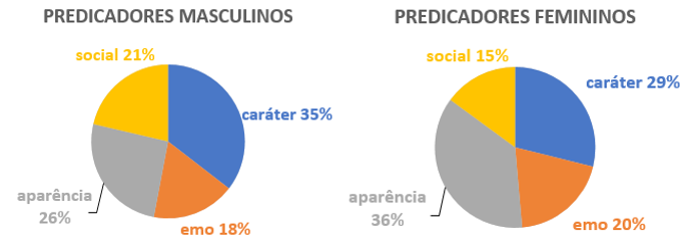
\includegraphics[width=0.85\textwidth]{Fig2.png}
 \caption{Distribuição das predicações humanas por gênero e por eixo.}
 \label{fig2}
 \source{Elaboração própria.}
\end{figure}

Considerando todo o acervo analisado, personagens masculinas são caracterizadas sobretudo pelo seu caráter/personalidade (35\%). Em seguida, temos a caracterização pela aparência (26\%), seguida de perto pelo papel social (21\%) e, por último, pelas emoções (18\%). Já personagens femininas caracterizam-se primariamente pela aparência (36\%), mas a distribuição é um pouco mais equilibrada que aquela apoiada nas 10 palavras mais frequentes. A caracterização por meio de traços de caráter (29\%) é a segunda mais comum e é curioso notar que aparência e caráter têm distribuições opostas para personagens masculinas e femininas. A caracterização feminina por meio de aspectos emocionais aparece na terceira posição (20\%) e, por último, temos o papel social (15\%), também diferindo da distribuição masculina.

Diminuindo a distância e aproximando novamente o olhar, podemos buscar, para cada categoria, os predicadores mais frequentes por gênero. A \Cref{tbl3} traz os 15 primeiros predicadores de cada classe.

\begin{table}[htbp]
\caption{Predicações masculinas e femininas, listadas por frequência.}
\label{tbl3}
\centering
\begin{tabular}{lp{5.75cm}p{5.75cm}}
\toprule
 & Predicações masculinas & Predicações femininas \\ \midrule
Emoção & 
Feliz, amigo, contente, alegre, valente*, atônito, amado, triste, espantado, pensativo, comovido, apaixonado, furioso, radiante, ansioso & 
Amada, feliz, alegre, amante*, triste, faceira*, trêmula, impaciente, amiga, assustada, agitada*, chorosa*, radiante, espantada, tranquila \\
Caráter & 
Bom, sério, grande, honesto, digno, capaz, inteligente, mau, honrado*, doido, grave*, valente*, generoso, frio, vulgar & 
Honesta, boa, perdida*, capaz, livre, vulgar, de verdade*, digna, impaciente*, fácil, indiferente, discreta, fresca, infame, inteligente \\
Aparência & 
Alto, magro, bonito, pálido, gordo, forte, velho, (homem)feito, moço, branco, doente, baixo, elegante, robusto, vestido &
Bonita, bela, pálida, formosa*, alta, feia, linda*, velha, loira, morena, vestida, encantadora*, forte, moça, nua \\
Papel & 
Rico, pobre, solteiro, público*, amigo, casado, filho, político*, capitão*, feiticeiro, notável*, português*, sertanejo, primitivo*, importante* &
Rica, casada, pobre, perdida, filha, viúva, solteira, mãe*, sozinha, amiga, distinta, empregada, guerreira*, feiticeira, virgem \\
\bottomrule
\end{tabular}
\source{Elaboração própria.}
\notes{As palavras com * referem-se a predicações usadas exclusivamente para aquele gênero no material de análise.}
\end{table}

Na categoria \textit{emoção}, as caracterizações femininas mais comuns remetem aos sentimentos de felicidade (\textit{feliz}, \textit{alegre}, \textit{radiante}, \textit{faceira}), tristeza (\textit{triste}, \textit{chorosa}), medo e surpresa (\textit{trêmula}, \textit{assustada}, \textit{agitada}, \textit{espantada}) e ao amor/amizade (amada, amante, amiga)\footnote{As palavras \textit{amante} e \textit{amiga} pertencem tanto à classe emoção quanto à caracterização social (amante em oposição à esposa, por exemplo). O segundo uso é mais frequente no \textit{corpus}, mas como não temos, por enquanto, este nível granular de análise, mantivemos as palavras nas duas classes.}. Já as características masculinas mais comuns também remetem aos sentimentos de felicidade (\textit{feliz}, \textit{contente} \textit{alegre}, \textit{radiante}), medo e surpresa (\textit{atônito}, \textit{espantado}) e amor/amizade (\textit{amigo}, \textit{amado}, \textit{apaixonado}), mas a tristeza comparece apenas com uma palavra (\textit{triste}). Além disso, vemos a presença do sentimento de coragem (\textit{valente}) ausente nas caracterizações femininas como um todo. As caracterizações emocionais exclusivamente femininas são mais variadas, indicando também que se quantitativamente a classe das emoções aproxima personagens masculinas e femininas, qualitativamente existem diferenças relacionadas ao gênero, cabendo às personagens femininas maior riqueza emocional.

Na categoria \textit{caráter}, as caracterizações femininas e masculinas mais comuns remetem a aspectos valorizados socialmente como honestidade, dignidade e bondade, mas também há muitas caracterizações negativas. No entanto, as caracterizações negativas masculinas (\textit{mau}, \textit{doido}, \textit{vulgar}) são menos variadas que as femininas (\textit{perdida}, \textit{vulgar}, \textit{fácil}, \textit{fresca}, \textit{infame}, \textit{impaciente}). Além disso, as caracterizações masculinas exclusivas, neste recorte, remetem ao que é socialmente valorizado (\textit{honrado}, \textit{grave}, \textit{valente}), enquanto as predicações femininas exclusivas são mais negativas (\textit{perdida}, \textit{impaciente}) que positivas (\textit{de verdade}).

Na categoria \textit{aparência}, retomamos a predominância da caracterização feminina por meio da beleza, explicitada pelo uso de itens lexicais variados (\textit{bonita}, \textit{bela}, \textit{formosa}, \textit{linda}, \textit{encantadora}), enquanto a beleza masculina aparece apenas em bonito (e, talvez, \textit{elegante}). É curioso notar que, na amostra, a classe aparência é a única que não tem caracterizações exclusivamente masculinas e, de maneira complementar, as caracterizações exclusivamente femininas são todas do campo da beleza (\textit{formosa}, \textit{linda}, \textit{encantadora}).

Por fim, na categoria relacionada ao \textit{papel social}, se tanto personagens masculinas quanto femininas podem ser \textit{ricos}, \textit{pobres}, \textit{solteiros}, \textit{casados}, \textit{filhos} e \textit{filhas}, mulheres são \textit{mães}, mas homens raramente são \textit{pais} (a frequência de \textit{pai} é três vezes menor que a de \textit{mãe} em um \textit{corpus} em que há mais personagens – e caracterizações – masculinas que femininas). Personagens femininas tendem a ter seu espaço social limitado à esfera familiar/doméstica (\textit{casada}, \textit{filha}, \textit{viúva}, \textit{solteira}, \textit{mãe}, \textit{sozinha}, \textit{amiga}), que também comparece nas caracterizações masculinas, mas de maneira mais modesta (\textit{solteiro}, \textit{amigo}, \textit{casado}, \textit{filho}). Caracterizações sociais masculinas, por sua vez, não se limitam à esfera doméstica, o que é reforçado pela constatação de que a maioria delas é usada exclusivamente para homens (\textit{homem público}, \textit{político}, \textit{capitão}).

\subsection{Uma leitura discursiva dos dados}\label{sec-formato}
Até aqui, apresentamos os resultados de uma leitura não-linear da caracterização de personagens em 233 obras literárias brasileiras do século XIX e primeira metade do século XX, tomando como eixo de análise o gênero. A partir da busca por estruturas predicadoras em um \textit{corpus} anotado morfossintaticamente, distinguimos quatro categorias de análise e distribuímos os dados por essas classes, o que nos ofereceu uma perspectiva produtiva para observar tendências (históricas, editoriais etc.), ampliando um tipo de análise que normalmente se restringe aos estudos de caso.

Resumidamente, temos como pistas até aqui: (i) fala-se mais de homens do que de mulheres (uma literatura feita por homens-autores); (ii) embora se prediquem mais homens que mulheres, a predicação feminina mais frequente (\textit{bonita}) repete-se muito mais (quase três vezes mais) que a masculina mais frequente (\textit{sério}); (iii) levando-se em conta os dados dispersos pela cauda longa, novamente se constata que personagens femininas são caracterizadas primariamente pela aparência, em seguida pelo caráter (essa relação aparece invertida para os homens), emoções/afeto em terceiro lugar e, por fim, o papel social (esse segundo par também aparece invertido nas predicações masculinas); (iv) apesar de a distribuição de todas as predicações apontar para um cenário mais equilibrado do que aquela que considera apenas as palavras mais frequentes, qualitativamente a natureza das predicações mostra algumas diferenças entre mulheres e homens: tomados em conjunto e analisados discursivamente, os números indexicalizam a invisibilidade da mulher enquanto elemento da sociedade e dotado de personalidade, em oposição, por exemplo, à imensa exposição de seus atributos físicos.

Esse retrato, disparado por uma leitura distante do \textit{corpus}, auxiliou-nos na identificação de como mulheres e homens são majoritariamente representados na literatura brasileira do período estudado. A partir de agora, recuperamos os vetores centrais comuns às análises discursivas – o caráter contextualmente situado, dialógico, performativo e indexical da linguagem – para tecer considerações mais atentas aos modos como uma leitura não-linear e distante pode coadunar uma análise discursiva.

Iniciamos retomando a constatação relativa à constituição do \textit{corpus}: temos apenas duas mulheres na lista de autores e 60\% das predicações são atribuídas a personagens masculinas. \textcite{maingueneau2006}, sobre a análise de textos literários, chama atenção para a necessidade de se considerar o “fato literário” também como acontecimento discursivo, cuja possibilidade de existência está associada às condições de comunicação literária e sua inscrição sócio-histórica. De fato, desde \textcite{foucault_ordem_2012}, compreendemos a produção e a circulação do discurso como institucionalmente organizados, selecionados e controlados por certos procedimentos que dominam suas aparições aleatórias.

Nesse âmbito, o trabalho de \textcite{underwood2018}, realizado na perspectiva das Humanidades Digitais, traz dados que ajudam a situar alguns de nossos resultados. Os autores analisam uma coleção de 104 mil obras ficcionais de língua inglesa cobrindo o período que vai de 1703 a 2009, sendo a maioria delas de 1780 a 2007. A partir dos dados, os autores apontam que a ficção de língua inglesa era dominada por escritoras no início do século XIX. De acordo com o trabalho, se até por volta de 1840 mulheres representavam quase metade dos autores de ficção, por volta de 1917 este número cai para quase um quarto. Segundo Tuchman e Fortin (2012, apud \cite{underwood2018}), o declínio pode ser explicado por alguns fatores: (i) o status que a profissão de romancista começa a ganhar após 1840 e uma melhora nas condições de trabalho dos romancistas, levando a uma “gentrificação” masculina do romance; (ii) pressões sociais no ambiente literário relativamente aos contratos das editoras, que sujeitaram mulheres a desvantagens crescentes no final do século XIX; (iii) a abertura, para as mulheres, de carreiras intelectuais diferentes da de romancista. Conforme os dados de \textcite{underwood2018} e levando em conta apenas as evidências de autoria, a ficção é uma das poucas “seções da biblioteca” onde a representação de mulheres parece ter diminuído.

Outro aspecto associado ao declínio do romance feminino de 1850 a 1940, ainda conforme \textcite{underwood2018}, manifesta-se no espaço que escritores reservam para homens ou mulheres ficcionais. Em livros escritos por homens, as mulheres ocupam em média apenas de um quarto a um terço do espaço dedicado a personagens masculinos. Nos livros escritos por mulheres, a divisão de espaço (em termos de números de palavras) é muito mais equilibrada. Essa lacuna entre os gêneros é estável ao longo de duzentos anos e está alinhada com a maior frequência de personagens (e predicações) masculinas em nosso material, composto por obras brasileiras. No entanto, segundo os autores, o declínio da proeminência das mulheres como personagens entre 1850 e 1960 permanece visível, ainda que de maneira sutil, mesmo após a separação dos volumes escritos por homens e mulheres, sugerindo que a sub-representação de personagens femininas não pode ser completamente explicada pela sub-representação de obras escritas por mulheres. O que temos, em resumo, é a necessidade de mais pesquisas na área e, quando voltamos ao nosso trabalho, mais ainda no que se refere ao contexto brasileiro.

Um olhar discursivo sobre os dados também trará para o centro da análise a dimensão lexical, aqui evidenciada por listas de predicadores humanos. Assim, é bastante comum que análise(s) de discurso se debruce(m) sobre as entradas lexicais dos textos que lhe(s) servem de objeto. Desde \textcite{bakhtin1979}, aposta-se na vinculação histórica e cultural entre os signos e um sentido “ideológico e vivencial”. Para o autor, em franca oposição a concepções de sentido que tomam a relação entre significante e significado como representacionais e estáveis, palavras são arenas de disputa e sua estabilidade aparente é resultado parcial e provisório de luta. Nessa esteira, \textcite{fairclough1992}\footnote{Não estamos optando aqui por uma outra corrente de análise discursiva, mas nos referindo a uma grade de ideias comum ao campo dos estudos discursivos. Por isso, optamos propositalmente por mesclar referências a expoentes de diversas tendências.}, na tentativa de formular maneiras de operacionalizar essa concepção sobre o signo em um tipo de análise orientada para textos concretos, elenca o léxico em geral e o modo como ele está a serviço de representar atores sociais em específico como uma entrada analítica útil para identificar as disputas sobre o sentido que derivam de processos culturais mais amplos. Nesse sentido, entradas lexicais, dentro ou fora de construções sintáticas predicadoras, são avaliativas.

Também para \textcite{possenti2004}, o léxico usado em discursos mapeia posições excludentes em formações discursivas \cite{foucault1969}. Pense-se, por exemplo, em como, no interior de uma mesma posição, a ocorrência em textos de imprensa de, digamos, \textit{invadir} rejeitaria a ocorrência de \textit{ocupar}. No âmbito do \textit{corpus} aqui escrutinado, por exemplo, \textit{chorosa} rejeita \textit{triste}. Embora ambas denotem tristeza, a dimensão sentimental e piegas está mais associada à primeira, que não por acaso aparece como predicador exclusivamente feminino na amostra que exploramos. No entanto, como indicamos, o OBras é um \textit{corpus} dinâmico, novas obras foram adicionadas, e uma busca recente por \textit{choroso} e \textit{chorosa} traz dados que corroboram as diferentes formações discursivas associadas a homens e mulheres. Assim, se com um material mais amplo constatamos que homens também podem ser \textit{chorosos}, a frequência com que o adjetivo é usado para qualificar homens é muitíssimo inferior àquela usada para mulheres.

De maneira complementar, a análise de cada caso por meio da leitura das linhas de concordância reforça a proposta de sinergia entre métodos qualitativos e quantitativos. Em outras palavras, olhamos de longe e, de lá, demarcamos regiões que podemos explorar detalhadamente. O movimento inverso, que parte da leitura convencional ou das linhas de concordância (baseadas apenas nas formas) seria praticamente impossível, ou seja, ler de maneira atenta quase 4 mil linhas de concordância, sendo mais da metade delas ocorrências de predicações únicas e dali selecionar questões para aprofundamento. A solução imediata – lidar apenas com o que é mais frequente – desconsidera mais da metade dos dados. As \Cref{fig3} e \Cref{fig4} trazem concordâncias de choroso e chorosa, respectivamente\footnote{Apesar de nos limitarmos, nas linhas de concordância, às frases que contém a palavra de interesse, é sempre possível expandir os contextos das frases.}.

\begin{figure}[htbp]
 \centering
 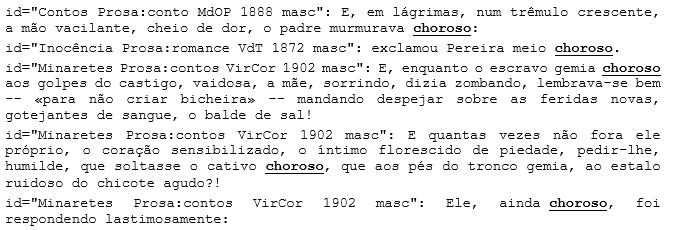
\includegraphics[width=0.85\textwidth]{Fig3.png}
 \caption{Linhas de concordância para a palavra \textit{choroso}.}
 \label{fig3}
 \source{Elaboração própria.}
\end{figure}

\begin{figure}[htbp]
 \centering
 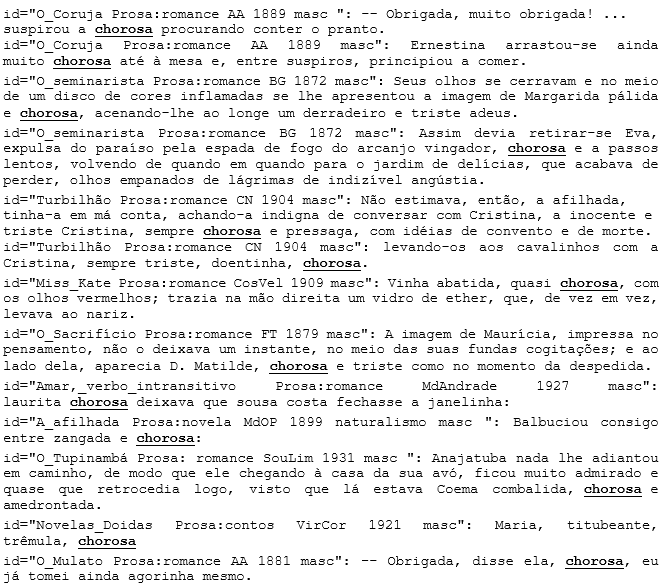
\includegraphics[width=0.85\textwidth]{Fig4.png}
 \caption{Linhas de concordância para a palavra \textit{chorosa}.}
 \label{fig4}
 \source{Elaboração própria.}
\end{figure}

Para boa parte das análises discursivas, a prática de \textit{wording} (nomear ou selecionar\footnote{Note-se que “escolha” aqui não quer dizer uma opção consciente da parte do enunciador do discurso.} palavras), mais do que \textit{revelar} ou \textit{representar} posições ideológicas dadas aprioristicamente, tem papel constitutivo, isto é, oferece existência a seres, relações, ações e \textit{propriedades} no mundo social e posiciona esses elementos em teias de disputa ideológica. Segundo \textcite{rajagopalan2010}, essa prática, que coloca essas entidades ou propriedades, que é o nosso foco aqui, “no centro do palco” e torna-as disponíveis “para práticas discursivas adicionais”, deve ser vista como o primeiro e talvez o passo mais importante na manipulação ideológica da atitude dos leitores em relação ao objeto nomeado e comentado, a partir de mecanismos de valoração disfarçados de descrição objetiva. Nesse sentido, uma análise que parte da comparação – qualitativa e quantitativa – entre predicadores por classe e gênero (conforme a \Cref{tbl3}) oferece um ponto de partida diferente para investigar as questões de pesquisa levantadas aqui, podendo se constituir em “apenas” um atalho ou em um percurso que leva a um novo ponto de chegada.

A noção de indexicalidade encapsula conceitualmente um dos pontos defendidos nos parágrafos anteriores, a saber, a ideia de que signos linguísticos – ou semióticos – se associam a repertórios culturais mais amplos \cite{silverstein1976}. A forma de predicar homens e mulheres na literatura brasileira do século XIX e início do século XX é índice de sistemas de crença, das formas de se estar e das possibilidades de se mover naquele (neste?) mundo. Especificamente, as predicações e as classificações exploradas nesse \textit{corpus} apontam, indiciam\footnote{Estamos cientes de que as relações de indexicalidade, por serem processos interpretativos, estão sujeitas aos repertórios variados dos interactantes.}, predominantemente, repertórios culturais que podemos chamar aqui de \textit{fisicalização}, \textit{fragilização} e \textit{domesticação} da mulher. Essas associações, por sua vez, estão sustentadas em posições ou sistemas de crenças sobre gênero, que, para dizer o óbvio, criam impressões de homogeneidade sobre a categoria \textit{mulher} e equacionam essa categoria com tropos de sensualidade, emotividade, passividade, maternidade etc.

O ponto a se destacar aqui é que a literatura do período selecionado não só é constituída, como é também constituinte das molduras regulatórias de gênero \cite{butler1990} que informam e fazem circular as imagens e performances masculinas e femininas até hoje, com destaque para a hiper-representação do corpo feminino e sub-representação de sua relevância socioeconômica e complexidade subjetiva. Em outras palavras, estamos tomando aqui a literatura (e não os autores em sua dimensão psicossocial) como coprodutora de realidade e cultura e, mais especificamente, estamos tomando a predicação como um dos elementos indexicais e fabricadores de gênero.

Os números e padrões encontrados na análise do \textit{corpus} operam esses mesmos efeitos. Especialmente via quantidade, uma \textit{diferenciação} \cite{thompsom1990} simbólica, regular e massiva, entre personagens masculinos e femininos é construída e, na esteira, alguns sentidos sobre o feminino são tornados mais visíveis, enquanto outros são obscurecidos. Os números nos fornecem pistas para as repetições desses sentidos, sinalizando a sua hegemonia nos embates sobre questões de gênero na literatura brasileira do período. Neste ponto, a frequência das formas importa, quer daquelas salientes pela repetição, quer daquelas invisibilizadas pela ocorrência única, mas trazidas à tona pela contagem.

Além disso, os textos literários, como qualquer acontecimento discursivo, são dialógicos \cite{bakthin1992}, no sentido de que projetam uma audiência, públicos e contrapúblicos e estão sempre em relação interdependente com outras práticas discursivas, vindas de esferas diferentes de atividade \cite{fairclough1992,foucault_ordem_2012}, isto é, esses textos participam de uma cadeia de outros discursos contemporâneos, passados e vindouros sobre o feminino e o masculino, afetando e sendo afetados por eles. Os textos literários que nos serviram de base, por exemplo, foram escritos por (e para) cidadãos nas esferas de poder, de dentro de sistemas de distribuição que investem nas obras de prestígio cultural e mantêm para elas uma circulação privilegiada até hoje – basta pensar em como essas obras participam de práticas educativas, por exemplo. A análise do texto literário, nas palavras de \textcite{mussalim2018}, é análise também desses outros textos, isto é, análise de como romances, por exemplo, “se baseiam, incorporam, recontextualizam, dialogam com outros textos” (MISOCZKY, 2005, p 133 apud \cite{mussalim2018}). 
É por isso que a literatura nos interessa como \textit{corpus} e fonte de pesquisa importante para observar a dinâmica histórica e social das questões de gênero – como todo discurso, o texto literário não fala apenas sobre ele mesmo, mas serve de observatório para outros discursos com os quais mantém relação dialógica\footnote{Esta análise, como se viu, ficou circunscrita às tendências mais visíveis nos dados, o que não quer dizer obviamente, que os dados não contenham relações de contradição, negação e dissenso.}.

\section{Considerações finais}\label{sec-modelo}
Neste trabalho, apresentamos uma tentativa de articulação entre o estudo com grandes corpora e análise do discurso, alternando lentes que nos afastam e nos aproximam do texto, buscando tirar o melhor proveito de cada uma delas. A análise tem o elemento \textit{gênero} como operador analítico e, se não chega a trazer conclusões inovadoras, tem o mérito de abrir um caminho para explorações futuras, partindo-se, por exemplo, dos eixos propostos. Não almeja a substituição de análises discursivas mais convencionais, mas uma parceria, capaz de oferecer materialidade a certas percepções e, em certos casos, respostas e pontos de vista diferentes.

Nossa contribuição é principalmente metodológica: ao embasar a análise em um grande acervo cuja leitura convencional, para a realização deste estudo, seria inviável, acreditamos ter apresentado (e motivado) a comunidade à aproximação – ou sinergia – já identificada em \textcite{baker2008} e reforçada em \textcite{friginal2020}.  No entanto, e como vantagem, ainda fazemos uso de material (i) público e (ii) linguisticamente anotado. O primeiro ponto viabiliza a reprodução da pesquisa (o que é diferente de reprodução das análises), uma atividade desejável mas nem sempre exequível no ambiente acadêmico, sobretudo nos estudos da linguagem. Já o segundo ponto, a anotação, permite análises mais precisas, tirando proveito de tudo o que pistas gramaticais são capazes de oferecer no que se refere ao(s) sentido(s).

Ao fim do trabalho, algumas outras possibilidades de exploração e pesquisa nos parecem instigantes: análises contrastivas com acervos de características distintas, quer quanto ao tipo de discurso, quanto ao recorte cronológico, espaço geográfico, autoria; do mesmo modo, a análise da distribuição das categorias ao longo do tempo. A partir da análise que apresentamos aqui, pode-se obter, por exemplo, um contraste mais preciso com obras não canônicas – como se dão as predicações quando temos autoras mulheres, ou autores de periféricos (negros, LGBTQIA+ etc.), ou como isso se dá na literatura contemporânea? Do mesmo modo, nos permite o contraste com outros discursos – como se dão as predicações na mídia impressa, por exemplo? E o quanto há de diferença quando o objeto são outras literaturas de língua portuguesa? Além disso, que outras questões insuspeitas, também de ordem cultural e ideológica, poderiam se beneficiar de \textit{insights} fornecidos por uma exploração de \textit{corpus} como a que aqui apresentamos? O que nos diria uma investigação sobre a relação entre lugar e gênero (lugares mais frequentados por homens que por mulheres), por exemplo?

A análise aqui apresentada é preliminar e muitas análises complementares poderiam ser realizadas considerando as obras em contexto macro e micro. Adicionar mais uma dimensão da predicação, por exemplo, indicando quem é o responsável pela atribuição de qualidade, seria altamente desejável. Identificar e explorar outros dispositivos da língua portuguesa para predicar, como a \textit{nomeação} humana (refugiados, imigrantes, brasileiros, estrangeiros, reis, presidentes, vendedores, mendigos, desempregados, bêbados...) traria ainda mais robustez às análises. Por fim, um mapeamento sobre a predicação em português (uma \textit{gramática da qualificação}) seria de imensa valia. A partir dos mesmos procedimentos efetuados aqui, pretendemos também investir em outras maneiras de investigar papeis femininos e masculinos em textos: personagens que ocupam a posição de sujeito (agentividade) ou de objeto (tema/passividade), e os tipos de verbos envolvidos, por exemplo, são maneiras de complementar a caracterização que iniciamos. Em trabalhos anteriores [anônimo], iniciamos a identificação semiautomática do discurso relatado, que possibilita investigar tanto o tipo de verbo de elocução associado às personagens (gritar, lamentar, concordar, discordar), quanto a frequência com que falam (ou silenciam), o que também enriquece a caracterização de personagens. O discurso relatado, aliás, é um operador promissor para a convergência que iniciamos aqui, dada sua alta frequência em gêneros variados, sobretudo na mídia impressa.

\printbibliography\label{sec-bib}
% if the text is not in Portuguese, it might be necessary to use the code below instead to print the correct ABNT abbreviations [s.n.], [s.l.]
%\begin{portuguese}
%\printbibliography[title={Bibliography}]
%\end{portuguese}


%full list: conceptualization,datacuration,formalanalysis,funding,investigation,methodology,projadm,resources,software,supervision,validation,visualization,writing,review
\begin{contributors}[sec-contributors]
\authorcontribution{Cláudia Freitas}[conceptualization,datacuration,methodology,writing]
\authorcontribution{Flávia Martins}[datacuration,investigation,writing]
\authorcontribution{Liana Biar}[conceptualization,datacuration,writing]
\end{contributors}


\appendix 
Para as buscar os predicadores femininos, utilizamos a seguinte expressão de busca na versão 5.3 do \textit{corpus} OBras:

\begin{lstlisting}[basicstyle=\small\ttfamily,columns=flexible,breaklines=true]
([pos="PROP.*" & func="SUBJ>"] [lema="ser|estar"] [pos="ADV.*"]* @[temcagr!=".*PASS.*" & pos="ADJ|N|V" & gen="F" & func="<SC"])|([pos="PROP.*"] "era" [pos="ADV.*"]* [pos="ADJ.*" & gen="F" & func!=">N"] [word="e"] @[pos="ADJ.*" & gen="F" & func!=">N"])|([lema="ela" & func="SUBJ>"] [lema="ser|estar"] [pos="ADV.*"]* @[temcagr!=".*PASS.*" & pos="ADJ|N|V" & gen="F" & func="<SC"])|([lema="ela" & func="SUBJ>"] [lema="ser|estar"] [pos="ADV.*"]* [temcagr!=".*PASS.*" & pos="ADJ|N|V" & gen="F" & func="<SC"] "e" @[temcagr!=".*PASS.*" & pos="ADJ|N|V" & gen="F"])|([lema="ela" & func="SUBJ>"]  [lema="ser|estar"] [pos="ADV.*"]* [temcagr!=".*PASS.*" & pos="ADJ|N|V" & gen="F" & func="<SC"] "," @[temcagr!=".*PASS.*" & pos="ADJ|N|V" & gen="F"])|([pos="PROP.*" & func!="P<"] "," [pos="ADV.*"]* @[func="N<PRED|.*APP.*" & gen="F" & pos="ADJ"])|([pos="PROP.*" & func!="P<"] "," [pos="ADV.*"]* [func="N<PRED|.*APP.*" & gen="F" & pos="ADJ"] "e" @[gen="F" & pos="ADJ"])|([lema="mulher|moça|rapariga|esposa"] @[pos="N|ADJ|V" & func="<PRED|<OC|N<"])|([lema="mulher|moça|rapariga|esposa"] [pos="N|ADJ|V" & func="<PRED|<OC|N<"] "," @[pos="ADJ" & gen="F"])|([lema="mulher|moça|rapariga|esposa"] [pos="N|ADJ|V" & func="<PRED|<OC|N<"] "e" @[pos="ADJ" & gen="F"])
\end{lstlisting}

Para buscar os predicadores masculinos, utilizamos a seguinte expressão de busca na versão 5.3 do \textit{corpus} OBras:

\begin{lstlisting}[basicstyle=\small\ttfamily,columns=flexible,breaklines=true]
([pos="PROP.*" & func="SUBJ>"] [lema="ser|estar"] [pos="ADV.*"]* @[temcagr!=".*PASS.*" & pos="ADJ|N|V" & gen="M" & func="<SC"])|([pos="PROP.*"] "era" [pos="ADV.*"]* [pos="ADJ.*" & gen="M" & func!=">N"] [word="e"] @[pos="ADJ.*" & gen="M" & func!=">N"])|([lema="ela" & func="SUBJ>"] [lema="ser|estar"] [pos="ADV.*"]* @[temcagr!=".*PASS.*" & pos="ADJ|N|V" & gen="M" & func="<SC"])|([lema="ela" & func="SUBJ>"] [lema="ser|estar"] [pos="ADV.*"]* [temcagr!=".*PASS.*" & pos="ADJ|N|V" & gen="M" & func="<SC"] "e" @[temcagr!=".*PASS.*" & pos="ADJ|N|V" & gen="M"])|([lema="ela" & func="SUBJ>"]  [lema="ser|estar"] [pos="ADV.*"]* [temcagr!=".*PASS.*" & pos="ADJ|N|V" & gen="M" & func="<SC"] "," @[temcagr!=".*PASS.*" & pos="ADJ|N|V" & gen="M"])|([pos="PROP.*" & func!="P<"] "," [pos="ADV.*"]* @[func="N<PRED|.*APP.*" & gen="M" & pos="ADJ"])|([pos="PROP.*" & func!="P<"] "," [pos="ADV.*"]* [func="N<PRED|.*APP.*" & gen="M" & pos="ADJ"] "e" @[gen="F" & pos="ADJ"])|([lema="homem|moço|rapaz|marido"] @[pos="N|ADJ|V" & func="<PRED|<OC|N<"])|([lema="homem|moço|rapaz|marido"] [pos="N|ADJ|V" & func="<PRED|<OC|N<"] "," @[pos="ADJ" & gen="M"])|([lema="homem|moço|rapaz|marido"] [pos="N|ADJ|V" & func="<PRED|<OC|N<"] "e" @[pos="ADJ" & gen="M"])
\end{lstlisting}

\end{document}

